\section{Simulation Analysis}
\label{sec:simulation}


For the simulation analysis we used Ngpice to simulate the AC/DC converter we had architectured. 


In this analysis we ran our model for 1000 moments and measured the output voltage which turned out to be exactly as expected(12 Volts). Afterwards we plotted the voltages in nodes 4 and 5 which correspond to the envelope detector voltage regulator voltages, respectively ~\ref{fig:ngspice3}. Additionally we plotted $$v5 - 12$$ and $$v4 - 12$$, and by doing so we are analysing the deviations. ~\ref{fig:ngspice31} We also calculated the ripple with Ngspice

\begin{table}[h]
  \centering
  \begin{tabular}{|l|r|}
    \hline    
    {\bf Name} & {\bf Value [A or V]} \\ \hline
    \input{op1_tab}
  \end{tabular}
  \caption{}
  \label{tab:tabela1}
\end{table}

\begin{table}[h]
  \centering
  \begin{tabular}{|l|r|}
    \hline    
    {\bf Name} & {\bf Value [A or V]} \\ \hline
    \input{op2_tab}
  \end{tabular}
  \caption{}
  \label{tab:tabela2}
\end{table}

\begin{figure}[h] \centering
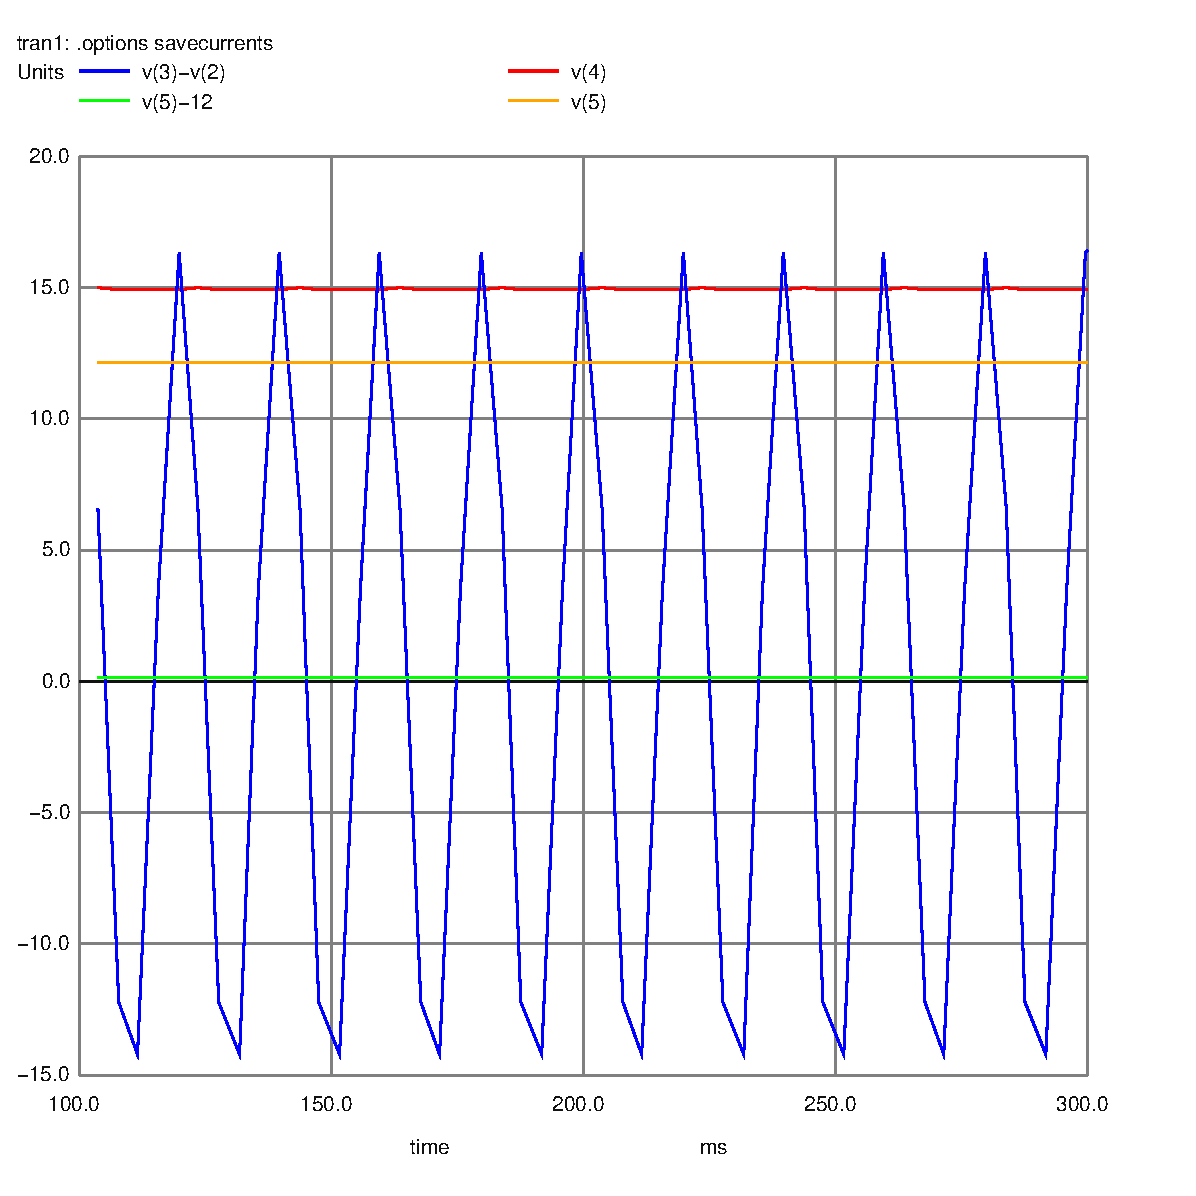
\includegraphics[width=0.8\linewidth]{ngspice3.eps}
\caption{Output Voltages of the Envelope Detector and Voltage Regulator.}
\label{fig:ngspice3}
\end{figure}

\begin{figure}[h] \centering
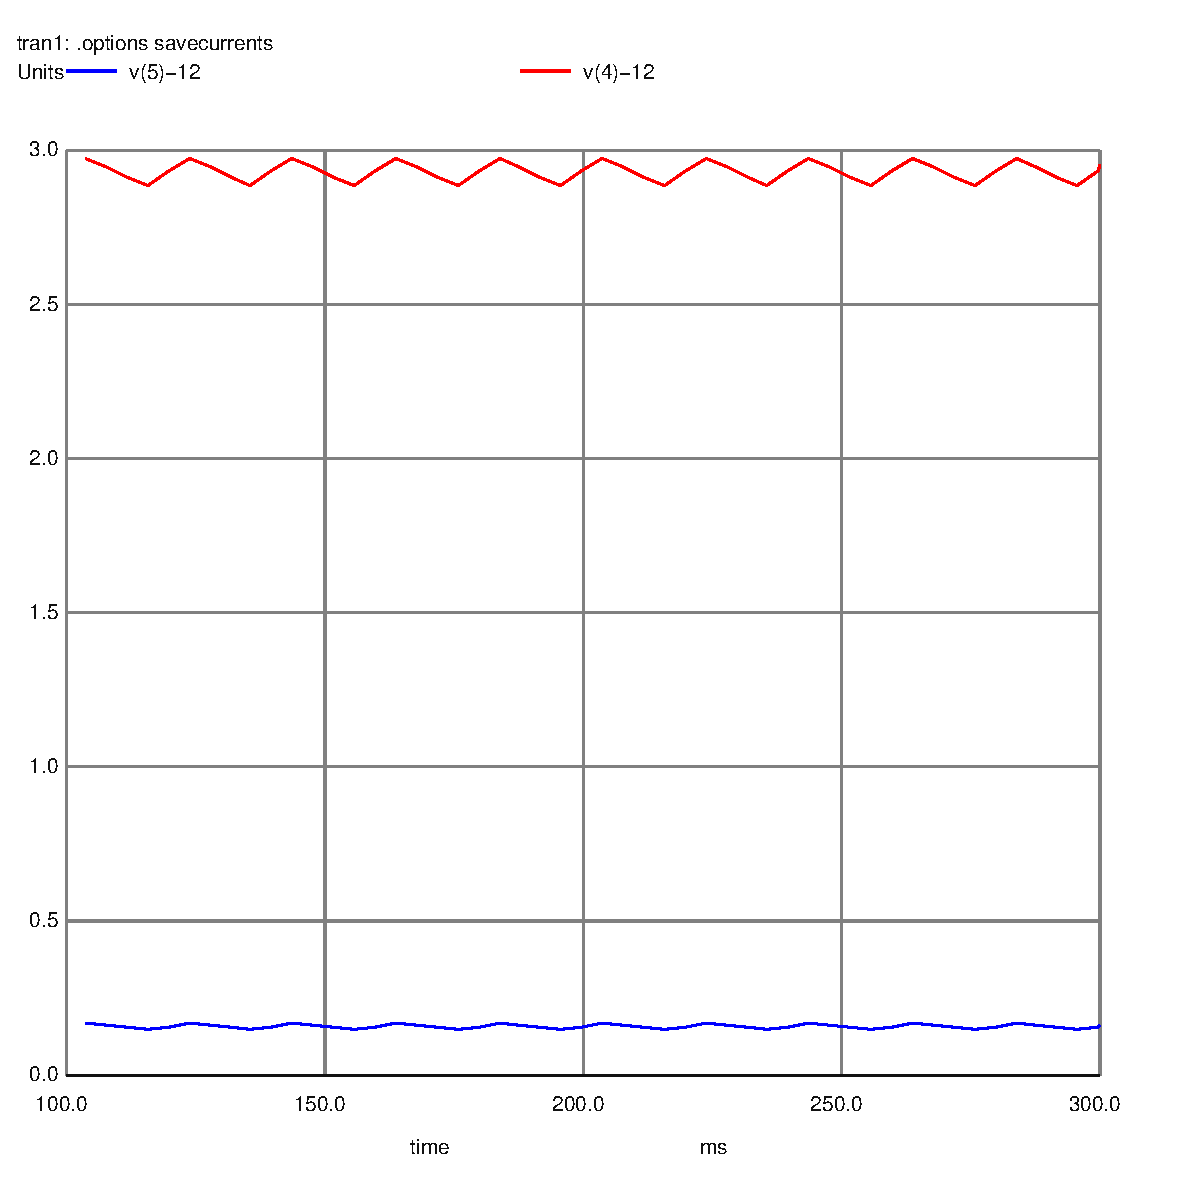
\includegraphics[width=0.8\linewidth]{ngspice31.eps}
\caption{Fluctuation of the output voltages for v4 and v5.}
\label{fig:ngspice31}
\end{figure}


All these results were expected and predicted in the theoretical section, as we can conclude by comparing the results in both plots.
